\documentclass{beamer}
\usetheme{CambridgeUS}
\usecolortheme{beaver}

\makeatletter
\defbeamertemplate*{title page}{mydefault}[1][]
{
	\vbox{}
	\vfill
	\begin{centering}

%{\usebeamercolor[fg]{titlegraphic}\inserttitlegraphic\par}
		\begin{beamercolorbox}{titlegraphic}
				\usebeamerfont{titlegraphic}\inserttitlegraphic
		\end{beamercolorbox}%
			\vskip1em\par	
		\begin{beamercolorbox}[rounded=true, center, shadow=true, sep=8pt,#1]{title}
			\usebeamerfont{title}\inserttitle\par%
			\ifx\insertsubtitle\@empty%
			\else%
			\vskip0.5em%
			{\usebeamerfont{subtitle}\usebeamercolor[fg]{subtitle}\insertsubtitle\par}%
			\fi%     
		\end{beamercolorbox}%
		\vskip1em\par
		\begin{beamercolorbox}[sep=8pt,center,#1]{author}
			\usebeamerfont{author}\insertauthor
		\end{beamercolorbox}
		\begin{beamercolorbox}[sep=8pt,center,#1]{institute}
			\usebeamerfont{institute}\insertinstitute
		\end{beamercolorbox}
		\begin{beamercolorbox}[sep=8pt,center,#1]{date}
			\usebeamerfont{date}\insertdate
		\end{beamercolorbox}\vskip0.5em
		\begin{beamercolorbox}[sep=8pt,center,#1]{logo}
			\usebeamerfont{titlegraphic}\insertlogo
		\end{beamercolorbox}%
	\end{centering}
	\vfill
}
\setbeamertemplate{title page}[mydefault]
\makeatother



\titlegraphic{
\includegraphics[width=50mm]{logo_dauphine} \hspace*{5.5cm} 
\includegraphics[width=7mm]{cnrs}}
\title[Elicitation and Explanation in Social Choice]{Elicitation and Explanation in Social Choice Theory}
%\subtitle{Proposal: ``Elicitation and Explanation for Voting Rules''}
\author[Beatrice Napolitano]{\textbf{Beatrice Napolitano} \\
	Supervisors: Remzi Sanver, Olivier Cailloux}
\date[JdL 18 April 2019]{Journée du LAMSADE \\ 18 April 2019 \\ 
\includegraphics[width=35mm]{LOGO_LAMSADE} }

\usepackage{tikz}
\usepackage{amsmath}
\usepackage{graphicx}
\newcommand{\ppref}{\succ^\text{p}}

\definecolor{darkred}{rgb}{0.8,0,0}

\begin{document}

\beamertemplatenavigationsymbolsempty

\begin{frame}[plain]
\maketitle
\end{frame}

\addtocounter{framenumber}{-1}


\section{Education and Experience}
\begin{frame}
	\frametitle{Education and Experience}
	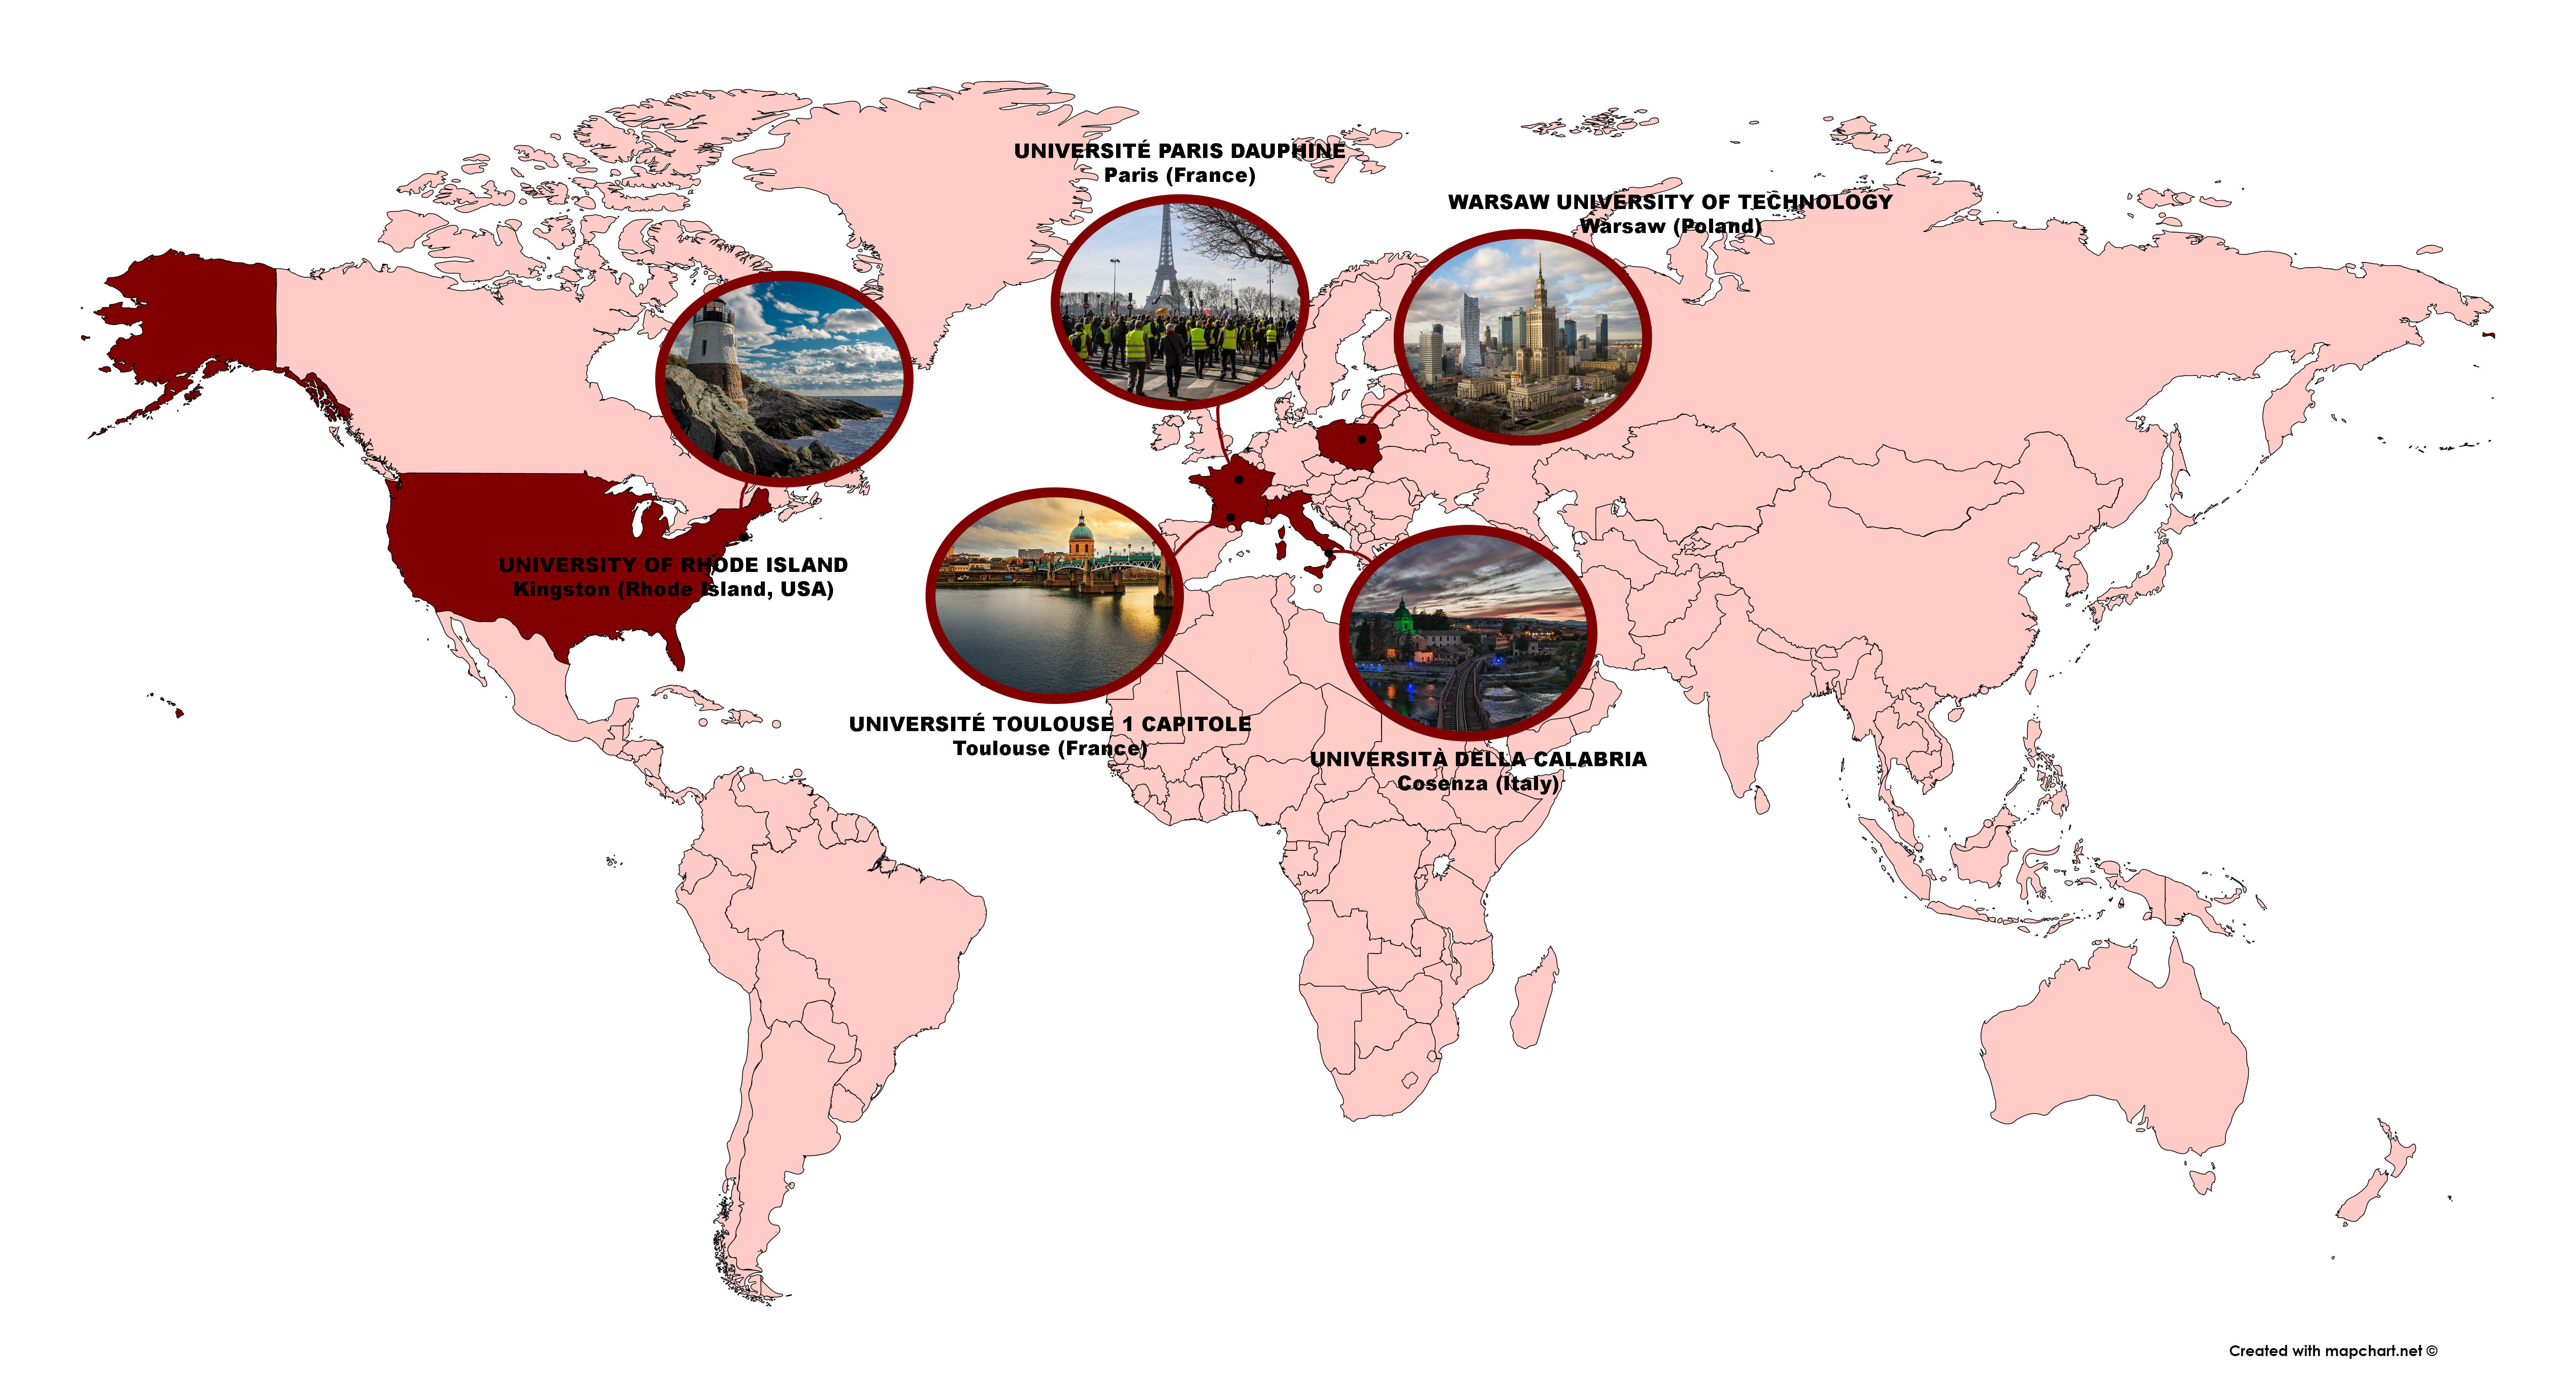
\includegraphics[width=\textwidth]{map}
\end{frame}

\section{Ph.D. Proposal}
\subsection*{Goal}
\begin{frame}
\frametitle{Ph.D. Proposal: \\ \textit{Elicitation and Explanation in Social Choice Theory}}
\framesubtitle{Goal}
Develop procedures able to help a committee (or a society) choose a suitable voting rule
\newline \newline \textbf{Involves}:
\begin{itemize}
	\item Axiomatic analysis of voting rules
	\item Explanation of axioms in non-expert terms
	\item Preference elicitation methods
\end{itemize}
\end{frame}


\section{Current Work}
\subsection{Minimax Regret}

\begin{frame}
\frametitle{Simultaneous Elicitation of Committee and Voters Preferences}
%\framesubtitle{Robust Winner Determination}
%	\textbf{Setting}: Two kind of players
\textbf{Setting}: Incomplete profile and uncertain scoring rule
\begin{figure}
	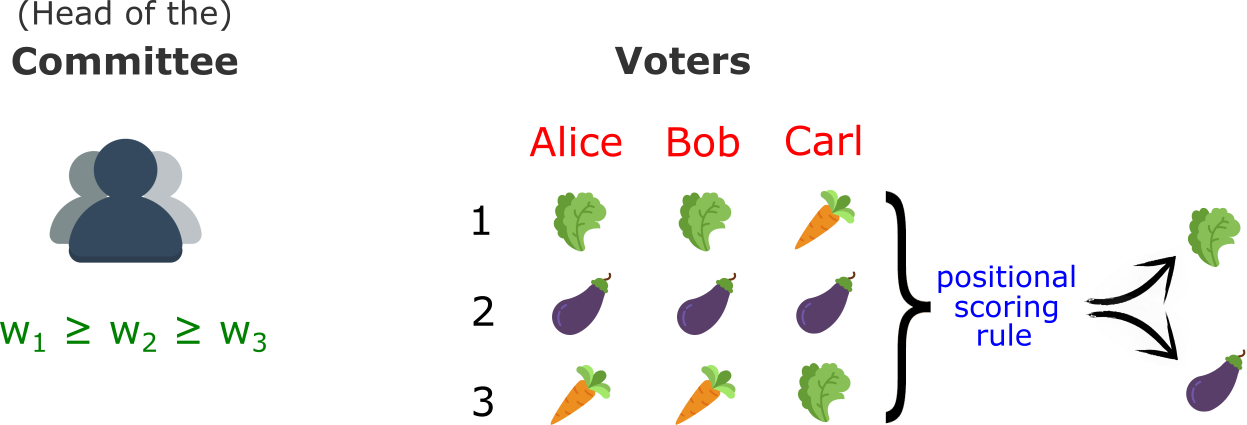
\includegraphics[scale=0.35]{set.png}
	%		\caption{.}
	%		\label{fig:b1}
\end{figure}
\textbf{Goal}: Winner determination using an incremental elicitation protocol based on minimax regret \\ \medskip {\scriptsize [\textit{Ongoing submission to RJCIA 2019}]}
\end{frame}
\addtocounter{framenumber}{-1}
\begin{frame}
	\frametitle{Simultaneous Elicitation of Committee and Voters Preferences}
	\textbf{Setting}: Incomplete profile and uncertain scoring rule
	\begin{figure}
		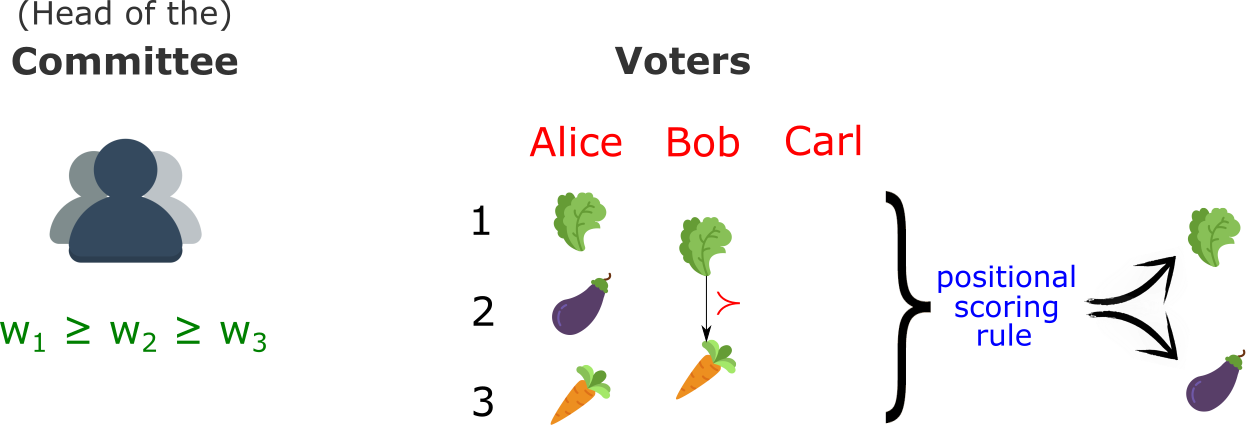
\includegraphics[scale=0.35]{set2.png}
%		\caption{.}
%		\label{fig:b1}
	\end{figure}
	\textbf{Goal}: Winner determination using an incremental elicitation protocol based on minimax regret \\ \medskip {\scriptsize [\textit{Ongoing submission to RJCIA 2019}]}
\end{frame}


\addtocounter{framenumber}{-1}
\begin{frame}[plain]
	\centering \color{darkred}\LARGE Thank You!
\end{frame}




\bibliographystyle{plain}
\bibliography{biblio} 
%given a combination of axioms we want to find an outcome that doesn't satisfy them, and we would do that for several reasons:
%-querying the user, depending of her answer we might infer her preferences over the set of axioms;
%-proving that a set of axioms is not valid giving a counter-example;


%A method for automatically proving impossibility theorems in the area of ranking sets of objects has already been implemented (Geist \& Endriss, 2011). It:



\end{document}